\documentclass{article}\usepackage[]{graphicx}\usepackage[]{color}
%% maxwidth is the original width if it is less than linewidth
%% otherwise use linewidth (to make sure the graphics do not exceed the margin)
\makeatletter
\def\maxwidth{ %
  \ifdim\Gin@nat@width>\linewidth
    \linewidth
  \else
    \Gin@nat@width
  \fi
}
\makeatother

\definecolor{fgcolor}{rgb}{0.345, 0.345, 0.345}
\newcommand{\hlnum}[1]{\textcolor[rgb]{0.686,0.059,0.569}{#1}}%
\newcommand{\hlstr}[1]{\textcolor[rgb]{0.192,0.494,0.8}{#1}}%
\newcommand{\hlcom}[1]{\textcolor[rgb]{0.678,0.584,0.686}{\textit{#1}}}%
\newcommand{\hlopt}[1]{\textcolor[rgb]{0,0,0}{#1}}%
\newcommand{\hlstd}[1]{\textcolor[rgb]{0.345,0.345,0.345}{#1}}%
\newcommand{\hlkwa}[1]{\textcolor[rgb]{0.161,0.373,0.58}{\textbf{#1}}}%
\newcommand{\hlkwb}[1]{\textcolor[rgb]{0.69,0.353,0.396}{#1}}%
\newcommand{\hlkwc}[1]{\textcolor[rgb]{0.333,0.667,0.333}{#1}}%
\newcommand{\hlkwd}[1]{\textcolor[rgb]{0.737,0.353,0.396}{\textbf{#1}}}%
\let\hlipl\hlkwb

\usepackage{framed}
\makeatletter
\newenvironment{kframe}{%
 \def\at@end@of@kframe{}%
 \ifinner\ifhmode%
  \def\at@end@of@kframe{\end{minipage}}%
  \begin{minipage}{\columnwidth}%
 \fi\fi%
 \def\FrameCommand##1{\hskip\@totalleftmargin \hskip-\fboxsep
 \colorbox{shadecolor}{##1}\hskip-\fboxsep
     % There is no \\@totalrightmargin, so:
     \hskip-\linewidth \hskip-\@totalleftmargin \hskip\columnwidth}%
 \MakeFramed {\advance\hsize-\width
   \@totalleftmargin\z@ \linewidth\hsize
   \@setminipage}}%
 {\par\unskip\endMakeFramed%
 \at@end@of@kframe}
\makeatother

\definecolor{shadecolor}{rgb}{.97, .97, .97}
\definecolor{messagecolor}{rgb}{0, 0, 0}
\definecolor{warningcolor}{rgb}{1, 0, 1}
\definecolor{errorcolor}{rgb}{1, 0, 0}
\newenvironment{knitrout}{}{} % an empty environment to be redefined in TeX

\usepackage{alltt}
\usepackage[letterpaper, portrait, margin=1in]{geometry}
\IfFileExists{upquote.sty}{\usepackage{upquote}}{}
\begin{document}
\title{Problem Set 4}
\author{Jeffrey Kwarsick}
\maketitle
\section{Problem 1}
\subsection{Part (a)}
The maximum number of copies that exist of vector 1:10 during the first execution of \emph{myFun()} is once.  From the code that I ran below, while invoking the \emph{.Internal(inspect())} commands, I was able to observe that the vector \emph{x} was passed into function x and since there was no operations conducted on the vector, the memory location is passed into the function \emph{f} and it's memory location is referenced as it is saved to the variable \emph{data}, located within the function.  When the vector is operated on within function \emph{f()} with function \emph{g()}, a copy is created within the local function environment and then the resulting vector from the operations of \emph{g()} is produced and outputed.  There is only a single copy because the vector is only being modified in a single spot, when operated on by function \emph{g()}.  A copy is made because objects in R are immutable, so to change them a copy is made locally within the function and the original is not modified.  After the operations are complete the copy of the vector is then deleted.
\par{Overall, this is an example of how R uses \emph{pass-by-value} in order to conduct operations of the function.  It makes a copy and executes operations on the copy of the object as needed rather than operating and modifying the original object.  This maintains the immutable nature of objects in R.  Specifically, this is referred as \emph{copy-on-change}.  This means that unless a change is made to the object, the function always references back to the original object, but when the function is going to make a change on the object, a copy is then made to carry out the operations.}
\begin{knitrout}
\definecolor{shadecolor}{rgb}{0.969, 0.969, 0.969}\color{fgcolor}\begin{kframe}
\begin{alltt}
\hlkwd{library}\hlstd{(}\hlstr{'pryr'}\hlstd{)}
\hlstd{x} \hlkwb{<-} \hlnum{1}\hlopt{:}\hlnum{10}
\hlkwd{.Internal}\hlstd{(}\hlkwd{inspect}\hlstd{(x))}
\end{alltt}
\begin{verbatim}
## @21cf590 13 INTSXP g0c4 [NAM(2)] (len=10, tl=0) 1,2,3,4,5,...
\end{verbatim}
\begin{alltt}
\hlstd{f} \hlkwb{<-} \hlkwa{function}\hlstd{(}\hlkwc{input}\hlstd{) \{}
  \hlkwd{.Internal}\hlstd{(}\hlkwd{inspect}\hlstd{(input))}
  \hlstd{data} \hlkwb{<-} \hlstd{input}
  \hlkwd{.Internal}\hlstd{(}\hlkwd{inspect}\hlstd{(data))}
  \hlstd{g} \hlkwb{<-} \hlkwa{function}\hlstd{(}\hlkwc{param}\hlstd{)} \hlkwd{return}\hlstd{(param} \hlopt{*} \hlstd{data)}
\hlstd{\}}
\hlstd{myFun} \hlkwb{<-} \hlkwd{f}\hlstd{(x)}
\end{alltt}
\begin{verbatim}
## @21cf590 13 INTSXP g0c4 [NAM(2)] (len=10, tl=0) 1,2,3,4,5,...
## @21cf590 13 INTSXP g0c4 [NAM(2)] (len=10, tl=0) 1,2,3,4,5,...
\end{verbatim}
\begin{alltt}
\hlkwd{.Internal}\hlstd{(}\hlkwd{inspect}\hlstd{(x))}
\end{alltt}
\begin{verbatim}
## @21cf590 13 INTSXP g0c4 [NAM(2)] (len=10, tl=0) 1,2,3,4,5,...
\end{verbatim}
\begin{alltt}
\hlstd{data} \hlkwb{<-} \hlnum{100}
\hlkwd{myFun}\hlstd{(}\hlnum{3}\hlstd{)}
\end{alltt}
\begin{verbatim}
##  [1]  3  6  9 12 15 18 21 24 27 30
\end{verbatim}
\begin{alltt}
\hlkwd{.Internal}\hlstd{(}\hlkwd{inspect}\hlstd{(}\hlkwd{myFun}\hlstd{(}\hlnum{3}\hlstd{)))}
\end{alltt}
\begin{verbatim}
## @2056718 14 REALSXP g0c5 [] (len=10, tl=0) 3,6,9,12,15,...
\end{verbatim}
\end{kframe}
\end{knitrout}
\subsection{Part (b)}
\begin{knitrout}
\definecolor{shadecolor}{rgb}{0.969, 0.969, 0.969}\color{fgcolor}\begin{kframe}
\begin{alltt}
\hlstd{x} \hlkwb{<-} \hlnum{1}\hlopt{:}\hlnum{10}
\hlstd{f} \hlkwb{<-} \hlkwa{function}\hlstd{(}\hlkwc{input}\hlstd{) \{}
  \hlstd{data} \hlkwb{<-} \hlstd{input}
  \hlstd{g} \hlkwb{<-} \hlkwa{function}\hlstd{(}\hlkwc{param}\hlstd{)} \hlkwd{return}\hlstd{(param} \hlopt{*} \hlstd{data)}
\hlstd{\}}
\hlstd{myFun} \hlkwb{<-} \hlkwd{f}\hlstd{(x)}
\hlkwd{object_size}\hlstd{(x)}
\end{alltt}
\begin{verbatim}
## 88 B
\end{verbatim}
\begin{alltt}
\hlkwd{length}\hlstd{(}\hlkwd{serialize}\hlstd{(x,} \hlkwa{NULL}\hlstd{))}
\end{alltt}
\begin{verbatim}
## [1] 62
\end{verbatim}
\begin{alltt}
\hlkwd{rm}\hlstd{(x)}
\hlkwd{object_size}\hlstd{(myFun)}
\end{alltt}
\begin{verbatim}
## 13.5 kB
\end{verbatim}
\begin{alltt}
\hlkwd{length}\hlstd{(}\hlkwd{serialize}\hlstd{(myFun,} \hlkwa{NULL}\hlstd{))}
\end{alltt}
\begin{verbatim}
## [1] 8505
\end{verbatim}
\begin{alltt}
\hlstd{data} \hlkwb{<-} \hlnum{100}
\hlkwd{myFun}\hlstd{(}\hlnum{3}\hlstd{)}
\end{alltt}
\begin{verbatim}
##  [1]  3  6  9 12 15 18 21 24 27 30
\end{verbatim}
\end{kframe}
\end{knitrout}
Running the chunk of code above with the to determine the size of \emph{myFun} and it's serialized length, I get a sizze of 2.53 kB and a length of 847.  This is done with a vector of range 1 - 10, of length 10.
\begin{knitrout}
\definecolor{shadecolor}{rgb}{0.969, 0.969, 0.969}\color{fgcolor}\begin{kframe}
\begin{alltt}
\hlstd{x1} \hlkwb{<-} \hlnum{1}\hlopt{:}\hlnum{10000}
\hlstd{f} \hlkwb{<-} \hlkwa{function}\hlstd{(}\hlkwc{input}\hlstd{) \{}
  \hlstd{data} \hlkwb{<-} \hlstd{input}
  \hlstd{g} \hlkwb{<-} \hlkwa{function}\hlstd{(}\hlkwc{param}\hlstd{)} \hlkwd{return}\hlstd{(param} \hlopt{*} \hlstd{data)}
\hlstd{\}}
\hlstd{myFun} \hlkwb{<-} \hlkwd{f}\hlstd{(x1)}
\hlkwd{object_size}\hlstd{(x1)}
\end{alltt}
\begin{verbatim}
## 40 kB
\end{verbatim}
\begin{alltt}
\hlkwd{length}\hlstd{(}\hlkwd{serialize}\hlstd{(x1,} \hlkwa{NULL}\hlstd{))}
\end{alltt}
\begin{verbatim}
## [1] 40022
\end{verbatim}
\begin{alltt}
\hlkwd{rm}\hlstd{(x1)}
\hlkwd{object_size}\hlstd{(myFun)}
\end{alltt}
\begin{verbatim}
## 53 kB
\end{verbatim}
\begin{alltt}
\hlkwd{length}\hlstd{(}\hlkwd{serialize}\hlstd{(myFun,} \hlkwa{NULL}\hlstd{))}
\end{alltt}
\begin{verbatim}
## [1] 88035
\end{verbatim}
\begin{alltt}
\hlstd{data} \hlkwb{<-} \hlnum{100}
\end{alltt}
\end{kframe}
\end{knitrout}
Running the same code again with a long vector of length ten thousand, with a range of 1 - 10000, I observe an object size of \emph{myFun} equal to 42.5 kB and a serialized length of 80768.
\subsection{Part (c)}
\begin{knitrout}
\definecolor{shadecolor}{rgb}{0.969, 0.969, 0.969}\color{fgcolor}\begin{kframe}
\begin{alltt}
\hlstd{x}  \hlkwb{<-} \hlnum{1}\hlopt{:}\hlnum{10}
\hlstd{f} \hlkwb{<-} \hlkwa{function}\hlstd{(}\hlkwc{data}\hlstd{) \{}
  \hlstd{g} \hlkwb{<-} \hlkwa{function}\hlstd{(}\hlkwc{param}\hlstd{)} \hlkwd{return}\hlstd{(param} \hlopt{*} \hlstd{data)}
  \hlkwd{return}\hlstd{(g)}
\hlstd{\}}
\hlstd{myFun} \hlkwb{<-} \hlkwd{f}\hlstd{(x)}
\hlkwd{rm}\hlstd{(x)}
\hlstd{data} \hlkwb{<-} \hlnum{100}
\hlkwd{myFun}\hlstd{(}\hlnum{3}\hlstd{)}
\end{alltt}


{\ttfamily\noindent\bfseries\color{errorcolor}{\#\# Error in myFun(3): object 'x' not found}}\end{kframe}
\end{knitrout}
The reason that the above code does not work is because the way objects are referenced and copied within a function environment.  R operates on a \emph{copy-on-change} basis.  This means that until a change is to be done on the object read into the list, it only references back to the original object.  When a change is to occur to the object, such as a multiplication or addition operation, a copy of the object is then made and the operations conducted.  In the case of the code above, the vector \emph{x} is called into function \emph{f()}, but is not operated on until the called in function \emph{g()}.  In the code chunk above, the original vecto \emph{x} is removed before the the parameter required to input into \emph{myFun} is called.  When \emph{myFun(3)} was called, there was no original object to reference back to and create a copy of and this is why the R reported that x was not found, because no copy of it was made in the local function environment before it was deleted.
\subsection{Part (d)}
\begin{knitrout}
\definecolor{shadecolor}{rgb}{0.969, 0.969, 0.969}\color{fgcolor}\begin{kframe}
\begin{alltt}
\hlstd{x} \hlkwb{<-} \hlnum{1}\hlopt{:}\hlnum{10}
\hlkwd{.Internal}\hlstd{(}\hlkwd{inspect}\hlstd{(x))}
\end{alltt}
\begin{verbatim}
## @2a6b7e8 13 INTSXP g0c4 [NAM(2)] (len=10, tl=0) 1,2,3,4,5,...
\end{verbatim}
\begin{alltt}
\hlstd{f} \hlkwb{<-} \hlkwa{function}\hlstd{(}\hlkwc{data}\hlstd{)\{}
  \hlstd{g} \hlkwb{<-} \hlkwa{function}\hlstd{(}\hlkwc{param}\hlstd{)} \hlkwd{return}\hlstd{(param} \hlopt{*} \hlstd{data)}
  \hlkwd{return}\hlstd{(g)}
\hlstd{\}}
\hlcom{#list the variables in the global environment}
\hlkwd{ls}\hlstd{(} \hlkwc{envir} \hlstd{= .GlobalEnv )}
\end{alltt}
\begin{verbatim}
## [1] "data"  "f"     "myFun" "x"
\end{verbatim}
\begin{alltt}
\hlstd{myFun} \hlkwb{<-} \hlkwd{f}\hlstd{(x)}
\hlcom{#stores pointer in the enclosed environment of the function myFun}
\hlkwd{environment}\hlstd{(myFun)}\hlopt{$}\hlstd{data}
\end{alltt}
\begin{verbatim}
##  [1]  1  2  3  4  5  6  7  8  9 10
\end{verbatim}
\begin{alltt}
\hlkwd{.Internal}\hlstd{(}\hlkwd{inspect}\hlstd{(}\hlkwd{environment}\hlstd{(myFun)}\hlopt{$}\hlstd{data))}
\end{alltt}
\begin{verbatim}
## @2a6b7e8 13 INTSXP g0c4 [MARK,NAM(2)] (len=10, tl=0) 1,2,3,4,5,...
\end{verbatim}
\begin{alltt}
\hlkwd{rm}\hlstd{(x)}
\hlkwd{ls}\hlstd{(} \hlkwc{envir} \hlstd{= .GlobalEnv )}
\end{alltt}
\begin{verbatim}
## [1] "data"  "f"     "myFun"
\end{verbatim}
\begin{alltt}
\hlkwd{object_size}\hlstd{(myFun)}
\end{alltt}
\begin{verbatim}
## 16.3 kB
\end{verbatim}
\begin{alltt}
\hlkwd{length}\hlstd{(}\hlkwd{serialize}\hlstd{(myFun,} \hlkwa{NULL}\hlstd{))}
\end{alltt}
\begin{verbatim}
## [1] 11102
\end{verbatim}
\begin{alltt}
\hlstd{data} \hlkwb{<-} \hlnum{100}
\hlkwd{myFun}\hlstd{(}\hlnum{3}\hlstd{)}
\end{alltt}
\begin{verbatim}
##  [1]  3  6  9 12 15 18 21 24 27 30
\end{verbatim}
\end{kframe}
\end{knitrout}
\noindent{In the code above, I am able to make the code from part (c) work without explicitly making a copy with the function body itself with the line of code \textbf{.Internal(inspect(environment(myFun)\$data))}.  In part (c) of the problem the \textbf{rm()} is called to remove x from the global environment in R.  With the line \textbf{.Internal(inspect(environment(myFun)\$data))}, the pointer pointing to the location in memory where x is stored and is saved to the enclosed environment of the function and thus is still able to be accessed despite the list x's removal from the global environment in R. Because there is no explicit copy made of x (as data) in the enclosed environment of \emph{myFun()}, the length of the serialized closure is considerably longer comapred to part (a) of the problem where an explicit copy of the vector is made.  The length is 10756.}
\section{Problem 2}
This problem was not done in RStudio, but a session of R in the terminal.  Code is written below to show what was done in order to complete the problem.
\subsection{Part (a)}
\begin{knitrout}
\definecolor{shadecolor}{rgb}{0.969, 0.969, 0.969}\color{fgcolor}\begin{kframe}
\begin{alltt}
\hlcom{#create a list of vectors}
\hlstd{list_of_vecs} \hlkwb{<-} \hlkwd{list}\hlstd{(}\hlkwd{c}\hlstd{(}\hlnum{1}\hlopt{:}\hlnum{3}\hlstd{),} \hlkwd{c}\hlstd{(}\hlnum{50}\hlopt{:}\hlnum{73}\hlstd{),} \hlkwd{c}\hlstd{(}\hlnum{22}\hlopt{:}\hlnum{45}\hlstd{))}
\hlcom{#Determine memory locations of the list and vectors within the list}
\hlkwd{.Internal}\hlstd{(}\hlkwd{inspect}\hlstd{(list_of_vecs))}
\end{alltt}
\begin{verbatim}
## @230d5f0 19 VECSXP g0c3 [NAM(2)] (len=3, tl=0)
##   @2778198 13 INTSXP g0c2 [] (len=3, tl=0) 1,2,3
##   @20bbab8 13 INTSXP g0c5 [] (len=24, tl=0) 50,51,52,53,54,...
##   @20bbc08 13 INTSXP g0c5 [] (len=24, tl=0) 22,23,24,25,26,...
\end{verbatim}
\begin{alltt}
\hlcom{#What is the size of the list of vectors}
\hlkwd{object_size}\hlstd{(list_of_vecs)}
\end{alltt}
\begin{verbatim}
## 464 B
\end{verbatim}
\begin{alltt}
\hlcom{#Change a single element within one of the vectors}
\hlstd{list_of_vecs[[}\hlnum{2}\hlstd{]][[}\hlnum{20}\hlstd{]]} \hlkwb{<-} \hlnum{169}
\hlcom{#Determine the memory locations and what changed}
\hlkwd{.Internal}\hlstd{(}\hlkwd{inspect}\hlstd{(list_of_vecs))}
\end{alltt}
\begin{verbatim}
## @2293e30 19 VECSXP g0c3 [NAM(1)] (len=3, tl=0)
##   @2778198 13 INTSXP g0c2 [NAM(2)] (len=3, tl=0) 1,2,3
##   @aa1b40 14 REALSXP g0c7 [] (len=24, tl=0) 50,51,52,53,54,...
##   @20bbc08 13 INTSXP g0c5 [NAM(2)] (len=24, tl=0) 22,23,24,25,26,...
\end{verbatim}
\end{kframe}
\end{knitrout}
When a change is made to an element within a vector within the list, a new vector is created of the vector where the change to the element was changed.  This is evident from the \textbf{.Internal(inspect())} command, revealing that the memory location of the vector where the change was made to an element was different compared to the memory locations before the changes was made.  In this case, R does not make the change in place.  It creates a copy of the vector being changed, makes the change to the element and then points to the new memory location where the changed vector resides.
\subsection{Part (b)}
\begin{knitrout}
\definecolor{shadecolor}{rgb}{0.969, 0.969, 0.969}\color{fgcolor}\begin{kframe}
\begin{alltt}
\hlcom{#Create a copy of list_of_vecs}
\hlstd{copy1} \hlkwb{<-} \hlstd{list_of_vecs}
\hlcom{#Determine memory locations of the copy}
\hlkwd{.Internal}\hlstd{(}\hlkwd{inspect}\hlstd{(copy1))}
\end{alltt}
\begin{verbatim}
## @2293e30 19 VECSXP g0c3 [MARK,NAM(2)] (len=3, tl=0)
##   @2778198 13 INTSXP g0c2 [MARK,NAM(2)] (len=3, tl=0) 1,2,3
##   @aa1b40 14 REALSXP g0c7 [MARK] (len=24, tl=0) 50,51,52,53,54,...
##   @20bbc08 13 INTSXP g0c5 [MARK,NAM(2)] (len=24, tl=0) 22,23,24,25,26,...
\end{verbatim}
\begin{alltt}
\hlcom{#Make a change to original list of vectors}
\hlstd{list_of_vecs[[}\hlnum{3}\hlstd{]][[}\hlnum{3}\hlstd{]]} \hlkwb{<-} \hlnum{72}
\hlcom{#Look at memory locations of both lists}
\hlcom{#of vectors}
\hlkwd{.Internal}\hlstd{(}\hlkwd{inspect}\hlstd{(list_of_vecs))}
\end{alltt}
\begin{verbatim}
## @1720d70 19 VECSXP g0c3 [NAM(1)] (len=3, tl=0)
##   @2778198 13 INTSXP g0c2 [MARK,NAM(2)] (len=3, tl=0) 1,2,3
##   @aa1b40 14 REALSXP g0c7 [MARK,NAM(2)] (len=24, tl=0) 50,51,52,53,54,...
##   @d70050 14 REALSXP g0c7 [] (len=24, tl=0) 22,23,72,25,26,...
\end{verbatim}
\begin{alltt}
\hlkwd{.Internal}\hlstd{(}\hlkwd{inspect}\hlstd{(copy1))}
\end{alltt}
\begin{verbatim}
## @2293e30 19 VECSXP g0c3 [MARK,NAM(2)] (len=3, tl=0)
##   @2778198 13 INTSXP g0c2 [MARK,NAM(2)] (len=3, tl=0) 1,2,3
##   @aa1b40 14 REALSXP g0c7 [MARK,NAM(2)] (len=24, tl=0) 50,51,52,53,54,...
##   @20bbc08 13 INTSXP g0c5 [MARK,NAM(2)] (len=24, tl=0) 22,23,24,25,26,...
\end{verbatim}
\end{kframe}
\end{knitrout}
Upon making a copy of the original list of vectors, the copy merely points to the memory locations of the original list of vectors.  Copy-on-change is occurring when the change is made to the original list of vectors.  The copy of the list of vectors maintains the same memory locations as shown by the two calls of the \textbf{.Internal(inspect())} of the copy of the list of vectors before and after a change is made to the original list of vectors.  In the original list of vectors, a copy of the vector changed within the list is made and the other vectors within the list maintain the same memory location, indicating they were not copied.
\subsection{Part (c)}
\begin{knitrout}
\definecolor{shadecolor}{rgb}{0.969, 0.969, 0.969}\color{fgcolor}\begin{kframe}
\begin{alltt}
\hlcom{#Create list of lists}
\hlstd{list_of_lists} \hlkwb{<-} \hlkwd{list}\hlstd{(}\hlkwd{list}\hlstd{(}\hlnum{1}\hlopt{:}\hlnum{25}\hlstd{),} \hlkwd{list}\hlstd{(}\hlnum{3}\hlopt{:}\hlnum{7}\hlstd{),} \hlkwd{list}\hlstd{(}\hlnum{90}\hlopt{:}\hlnum{100}\hlstd{))}
\hlcom{#Make copy of list}
\hlstd{copy2} \hlkwb{<-} \hlstd{list_of_lists}
\hlcom{#Look at the memory locations of original and copy}
\hlkwd{.Internal}\hlstd{(}\hlkwd{inspect}\hlstd{(list_of_lists))}
\end{alltt}
\begin{verbatim}
## @1720a58 19 VECSXP g0c3 [NAM(2)] (len=3, tl=0)
##   @2494178 19 VECSXP g0c1 [] (len=1, tl=0)
##     @2b10ad8 13 INTSXP g0c5 [] (len=25, tl=0) 1,2,3,4,5,...
##   @24941a8 19 VECSXP g0c1 [] (len=1, tl=0)
##     @1720a10 13 INTSXP g0c3 [] (len=5, tl=0) 3,4,5,6,7
##   @24941d8 19 VECSXP g0c1 [] (len=1, tl=0)
##     @2579138 13 INTSXP g0c4 [] (len=11, tl=0) 90,91,92,93,94,...
\end{verbatim}
\begin{alltt}
\hlkwd{.Internal}\hlstd{(}\hlkwd{inspect}\hlstd{(copy2))}
\end{alltt}
\begin{verbatim}
## @1720a58 19 VECSXP g0c3 [NAM(2)] (len=3, tl=0)
##   @2494178 19 VECSXP g0c1 [] (len=1, tl=0)
##     @2b10ad8 13 INTSXP g0c5 [] (len=25, tl=0) 1,2,3,4,5,...
##   @24941a8 19 VECSXP g0c1 [] (len=1, tl=0)
##     @1720a10 13 INTSXP g0c3 [] (len=5, tl=0) 3,4,5,6,7
##   @24941d8 19 VECSXP g0c1 [] (len=1, tl=0)
##     @2579138 13 INTSXP g0c4 [] (len=11, tl=0) 90,91,92,93,94,...
\end{verbatim}
\begin{alltt}
\hlcom{#Add element to copy of list_of_lists}
\hlstd{copy2[[}\hlnum{2}\hlstd{]][[}\hlnum{1}\hlstd{]]} \hlkwb{<-} \hlkwd{append}\hlstd{(copy2[[}\hlnum{2}\hlstd{]][[}\hlnum{1}\hlstd{]],} \hlnum{1001}\hlstd{)}
\hlcom{#Look at the memory locations of original and copy}
\hlcom{#After adding element to copy2}
\hlkwd{.Internal}\hlstd{(}\hlkwd{inspect}\hlstd{(list_of_lists))}
\end{alltt}
\begin{verbatim}
## @1720a58 19 VECSXP g0c3 [NAM(2)] (len=3, tl=0)
##   @2494178 19 VECSXP g0c1 [NAM(2)] (len=1, tl=0)
##     @2b10ad8 13 INTSXP g0c5 [] (len=25, tl=0) 1,2,3,4,5,...
##   @24941a8 19 VECSXP g0c1 [NAM(2)] (len=1, tl=0)
##     @1720a10 13 INTSXP g0c3 [NAM(2)] (len=5, tl=0) 3,4,5,6,7
##   @24941d8 19 VECSXP g0c1 [NAM(2)] (len=1, tl=0)
##     @2579138 13 INTSXP g0c4 [] (len=11, tl=0) 90,91,92,93,94,...
\end{verbatim}
\begin{alltt}
\hlkwd{.Internal}\hlstd{(}\hlkwd{inspect}\hlstd{(copy2))}
\end{alltt}
\begin{verbatim}
## @29bd5f0 19 VECSXP g0c3 [NAM(1)] (len=3, tl=0)
##   @2494178 19 VECSXP g0c1 [NAM(2)] (len=1, tl=0)
##     @2b10ad8 13 INTSXP g0c5 [] (len=25, tl=0) 1,2,3,4,5,...
##   @16f4fe8 19 VECSXP g0c1 [] (len=1, tl=0)
##     @246cc80 14 REALSXP g0c4 [NAM(2)] (len=6, tl=0) 3,4,5,6,7,...
##   @24941d8 19 VECSXP g0c1 [NAM(2)] (len=1, tl=0)
##     @2579138 13 INTSXP g0c4 [] (len=11, tl=0) 90,91,92,93,94,...
\end{verbatim}
\end{kframe}
\end{knitrout}
After creating a list of lists and then adding an element to the second list contained within the copy of the list of lists, I found that first and third lists that were unchanged between the copy and the original, were shared between the original and the copy of the list of lists.  The second lists between the original and the copy are different, indicating that it was copied in order append an element to the end of the second list within the copy.  The memory locations of the entire original list is different compared to copy.  This indicates that copy of the list was copied to a new memory location when the change was made.
\subsection{Part (d)}
While the overall size of \textbf{tmp} is 160 MB according to \emph{object.size(tmp)}, but from invoking \emph{gc()} I observe that only 80 MB is used.  When I invoke \emph{.Internal(inspec(tmp))}, I see that that both elements in tmp point to the same memory location.  This makes sense because both elements in \textbf{tmp} are comprised of the list of numbers, \emph{x}.  Thus, while the total size of \emph{tmp} may be 160 MB, R only uses 80 MB because both elements within \textbf{tmp} point to the memory location where \emph{x} is stored.
\section{Problem 3}
\begin{knitrout}
\definecolor{shadecolor}{rgb}{0.969, 0.969, 0.969}\color{fgcolor}\begin{kframe}
\begin{alltt}
\hlkwd{load}\hlstd{(}\hlstr{'ps4prob3.Rda'}\hlstd{)} \hlcom{# should have A, n, K}
\hlkwd{library}\hlstd{(}\hlstr{"microbenchmark"}\hlstd{)}
\hlcom{# Generates the log likelihood}
\hlstd{ll} \hlkwb{<-} \hlkwa{function}\hlstd{(}\hlkwc{Theta}\hlstd{,} \hlkwc{A}\hlstd{) \{}
  \hlstd{sum.ind} \hlkwb{<-} \hlkwd{which}\hlstd{(A}\hlopt{==}\hlnum{1}\hlstd{,} \hlkwc{arr.ind}\hlstd{=T)}
  \hlstd{logLik} \hlkwb{<-} \hlkwd{sum}\hlstd{(}\hlkwd{log}\hlstd{(Theta[sum.ind]))} \hlopt{-} \hlkwd{sum}\hlstd{(Theta)}
  \hlkwd{return}\hlstd{(logLik)}
\hlstd{\}}
\hlcom{#Original Code}
\hlstd{oneUpdate} \hlkwb{<-} \hlkwa{function}\hlstd{(}\hlkwc{A}\hlstd{,} \hlkwc{n}\hlstd{,} \hlkwc{K}\hlstd{,} \hlkwc{theta.old}\hlstd{,} \hlkwc{thresh} \hlstd{=} \hlnum{0.1}\hlstd{) \{}
  \hlstd{theta.old1} \hlkwb{<-} \hlstd{theta.old}
  \hlstd{Theta.old} \hlkwb{<-} \hlstd{theta.old} \hlopt \hlkwd{t}\hlstd{(theta.old)}
  \hlstd{L.old} \hlkwb{<-} \hlkwd{ll}\hlstd{(Theta.old, A)}
  \hlstd{q} \hlkwb{<-} \hlkwd{array}\hlstd{(}\hlnum{0}\hlstd{,} \hlkwc{dim} \hlstd{=} \hlkwd{c}\hlstd{(n, n, K))}
  \hlkwa{for} \hlstd{(i} \hlkwa{in} \hlnum{1}\hlopt{:}\hlstd{n) \{}
    \hlkwa{for} \hlstd{(j} \hlkwa{in} \hlnum{1}\hlopt{:}\hlstd{n) \{}
      \hlkwa{for} \hlstd{(z} \hlkwa{in} \hlnum{1}\hlopt{:}\hlstd{K) \{}
      \hlkwa{if} \hlstd{(theta.old[i, z]}\hlopt{*}\hlstd{theta.old[j, z]} \hlopt{==} \hlnum{0}\hlstd{) \{}
        \hlstd{q[i, j, z]} \hlkwb{<-} \hlnum{0}
        \hlstd{\}}
      \hlkwa{else} \hlstd{\{}
        \hlstd{q[i, j, z]} \hlkwb{<-} \hlstd{theta.old[i, z]}\hlopt{*}\hlstd{theta.old[j, z]} \hlopt{/}
            \hlstd{Theta.old[i, j]}
        \hlstd{\}}
      \hlstd{\}}
    \hlstd{\}}
  \hlstd{\}}
  \hlstd{theta.new} \hlkwb{<-} \hlstd{theta.old}
  \hlkwa{for} \hlstd{(z} \hlkwa{in} \hlnum{1}\hlopt{:}\hlstd{K) \{}
    \hlstd{theta.new[,z]} \hlkwb{<-} \hlkwd{rowSums}\hlstd{(A}\hlopt{*}\hlstd{q[,,z])}\hlopt{/}\hlkwd{sqrt}\hlstd{(}\hlkwd{sum}\hlstd{(A}\hlopt{*}\hlstd{q[,,z]))}
  \hlstd{\}}
  \hlstd{Theta.new} \hlkwb{<-} \hlstd{theta.new} \hlopt \hlkwd{t}\hlstd{(theta.new)}
  \hlstd{L.new} \hlkwb{<-} \hlkwd{ll}\hlstd{(Theta.new, A)}
  \hlstd{converge.check} \hlkwb{<-} \hlkwd{abs}\hlstd{(L.new} \hlopt{-} \hlstd{L.old)} \hlopt{<} \hlstd{thresh}
  \hlstd{theta.new} \hlkwb{<-} \hlstd{theta.new}\hlopt{/}\hlkwd{rowSums}\hlstd{(theta.new)}
  \hlkwd{return}\hlstd{(}\hlkwd{list}\hlstd{(}\hlkwc{theta} \hlstd{= theta.new,} \hlkwc{loglik} \hlstd{= L.new,}
              \hlkwc{converged} \hlstd{= converge.check))}
\hlstd{\}}
\hlcom{#Updated version of the function}
\hlcom{#Same initial conditions starting up}
\hlstd{oneUpdate.new.new} \hlkwb{<-} \hlkwa{function}\hlstd{(}\hlkwc{A}\hlstd{,} \hlkwc{n}\hlstd{,} \hlkwc{K}\hlstd{,} \hlkwc{theta.old}\hlstd{,} \hlkwc{thresh} \hlstd{=} \hlnum{0.1}\hlstd{) \{}
  \hlstd{theta.old1} \hlkwb{<-} \hlstd{theta.old}
  \hlstd{Theta.old} \hlkwb{<-} \hlstd{theta.old} \hlopt \hlkwd{t}\hlstd{(theta.old)}
  \hlstd{L.old} \hlkwb{<-} \hlkwd{ll}\hlstd{(Theta.old, A)}
  \hlstd{q} \hlkwb{<-} \hlkwd{array}\hlstd{(}\hlnum{0}\hlstd{,} \hlkwc{dim} \hlstd{=} \hlkwd{c}\hlstd{(n, n, K))}
  \hlstd{q.new} \hlkwb{<-} \hlkwd{array}\hlstd{(}\hlnum{0}\hlstd{,} \hlkwc{dim} \hlstd{=} \hlkwd{c}\hlstd{(n, n))}

  \hlstd{theta.new} \hlkwb{<-} \hlstd{theta.old}
  \hlcom{#Instead of running with 3 for-loops, creating a multi-dimensional space}
  \hlcom{#for performing the necessary calculations}
  \hlcom{#Invoking the kroeneker product yields the same matrix }
  \hlcom{#No conditional checks as well}
  \hlkwa{for} \hlstd{(z} \hlkwa{in} \hlnum{1}\hlopt{:}\hlstd{K) \{}
        \hlcom{# q.new <- theta.old[1:n,z] * theta.old[1:n,z] / Theta.old[1:n,1:n]}
    \hlstd{q.new} \hlkwb{<-} \hlkwd{matrix}\hlstd{(}\hlkwd{kronecker}\hlstd{(theta.old[}\hlnum{1}\hlopt{:}\hlstd{n,z], theta.old[}\hlnum{1}\hlopt{:}\hlstd{n,z]),} \hlkwc{nrow} \hlstd{= n,} \hlkwc{ncol} \hlstd{= n)} \hlopt{/}
      \hlstd{Theta.old}

    \hlstd{theta.new[,z]} \hlkwb{<-} \hlkwd{rowSums}\hlstd{(A}\hlopt{*}\hlstd{q.new)}\hlopt{/}\hlkwd{sqrt}\hlstd{(}\hlkwd{sum}\hlstd{(A}\hlopt{*}\hlstd{q.new))}
  \hlstd{\}}
  \hlcom{#same as the original code}
  \hlstd{Theta.new} \hlkwb{<-} \hlstd{theta.new} \hlopt \hlkwd{t}\hlstd{(theta.new)}
  \hlstd{L.new} \hlkwb{<-} \hlkwd{ll}\hlstd{(Theta.new, A)}
  \hlstd{converge.check} \hlkwb{<-} \hlkwd{abs}\hlstd{(L.new} \hlopt{-} \hlstd{L.old)} \hlopt{<} \hlstd{thresh}
  \hlstd{theta.new} \hlkwb{<-} \hlstd{theta.new}\hlopt{/}\hlkwd{rowSums}\hlstd{(theta.new)}
  \hlkwd{return}\hlstd{(}\hlkwd{list}\hlstd{(}\hlkwc{theta} \hlstd{= theta.new,} \hlkwc{loglik} \hlstd{= L.new,}
              \hlkwc{converged} \hlstd{= converge.check))}
\hlstd{\}}

\hlcom{#initialize the parameters at random starting values}
\hlstd{temp} \hlkwb{<-} \hlkwd{matrix}\hlstd{(}\hlkwd{runif}\hlstd{(n}\hlopt{*}\hlstd{K), n, K)}
\hlstd{theta.init} \hlkwb{<-} \hlstd{temp}\hlopt{/}\hlkwd{rowSums}\hlstd{(temp)}

\hlcom{#Proof of timing}
\hlkwd{microbenchmark}\hlstd{(}\hlkwd{oneUpdate}\hlstd{(A, n, K, theta.init),} \hlkwc{times}\hlstd{=}\hlnum{2}\hlstd{)}
\end{alltt}
\begin{verbatim}
## Unit: seconds
##                            expr      min       lq     mean   median
##  oneUpdate(A, n, K, theta.init) 79.99035 79.99035 80.95384 80.95384
##        uq      max neval
##  81.91733 81.91733     2
\end{verbatim}
\begin{alltt}
\hlkwd{microbenchmark}\hlstd{(}\hlkwd{oneUpdate.new.new}\hlstd{(A, n, K, theta.init),} \hlkwc{times}\hlstd{=}\hlnum{2}\hlstd{)}
\end{alltt}
\begin{verbatim}
## Unit: seconds
##                                    expr      min       lq     mean
##  oneUpdate.new.new(A, n, K, theta.init) 1.228801 1.228801 1.230336
##    median      uq     max neval
##  1.230336 1.23187 1.23187     2
\end{verbatim}
\begin{alltt}
\hlstd{a} \hlkwb{<-} \hlkwd{oneUpdate}\hlstd{(A, n, K, theta.init)}
\hlstd{c} \hlkwb{<-} \hlkwd{oneUpdate.new.new}\hlstd{(A, n, K, theta.init)}

\hlcom{#Proof of identity}
\hlkwd{table}\hlstd{(}\hlkwd{unlist}\hlstd{(a}\hlopt{$}\hlstd{theta} \hlopt{-} \hlstd{c}\hlopt{$}\hlstd{theta))}
\end{alltt}
\begin{verbatim}
## 
##     0 
## 50500
\end{verbatim}
\end{kframe}
\end{knitrout}
The issue with the original code is the iteration over three for-loops to process the large matrix required for the optimization of the statisical model.  The original code requires that the array is generated by iterating over each of the points in the generated array.  This stepwise fashion, coupled with the conditional checks at each indice within the array, results in the long computation time for a single iteration of the code, let alone multiple callings of the \emph{oneUpdate()} function required for the full optimzation of the problem.  The final for-loop that is used to go over the array again to complete the optimzation check steps further increases the computation time required for the execution of this function.
\par{This function can be improved with the elimination of the three nested for-loops and replaced with the invoking of the kroeneker product.  The Kroeneker product conducts the same multiplcation as is being done within the for-loops of the original function, but it does not require the iteration over every indice of the large array.  Being a function already present within R, invoking kroeneker to generate the necessary array required for the optimization, it already has an optimized efficiency for handling computation of large arrays/matrices.  This reduces all the three nested for-loops to a single for-loop to iterate over.}
\par{The new version of the function is compared with old function in terms of computational time and is checked in order to determine that the new function was able to generate the same function as the original.  From the microbenchmark check, the new function is considerably more efficient at completing the task and also results in the same matrix/array generated by the original function.}
\section{Problem 4}
I chose to modify PIKK in order to attempt an improvement of the efficiency of this algorithm.  The original function is below.
\begin{knitrout}
\definecolor{shadecolor}{rgb}{0.969, 0.969, 0.969}\color{fgcolor}\begin{kframe}
\begin{alltt}
\hlkwd{library}\hlstd{(}\hlstr{"microbenchmark"}\hlstd{)}
\hlstd{vec} \hlkwb{<-} \hlkwd{rnorm}\hlstd{(}\hlnum{1e5}\hlstd{)}
\hlstd{k} \hlkwb{<-} \hlnum{500}
\hlstd{PIKK} \hlkwb{<-} \hlkwa{function}\hlstd{(}\hlkwc{x}\hlstd{,} \hlkwc{k}\hlstd{) \{}
  \hlstd{x[}\hlkwd{sort}\hlstd{(}\hlkwd{runif}\hlstd{(}\hlkwd{length}\hlstd{(x)),} \hlkwc{index.return} \hlstd{=} \hlnum{TRUE}\hlstd{)}\hlopt{$}\hlstd{ix[}\hlnum{1}\hlopt{:}\hlstd{k]]}
\hlstd{\}}
\hlkwd{microbenchmark}\hlstd{(}\hlkwd{PIKK}\hlstd{(vec,k))}
\end{alltt}
\begin{verbatim}
## Unit: milliseconds
##          expr      min       lq     mean  median       uq      max neval
##  PIKK(vec, k) 24.77533 25.34225 25.69916 25.6156 26.11165 28.06241   100
\end{verbatim}
\end{kframe}
\end{knitrout}
In the original version of PIKK, the vector is taken and it's length used to generate a vector of random deviates of a uniform distribution.  This new vector is then sorted and the sorted indexes of this new list are used to pick \emph{k} from the population, in this case the input vector, \emph{vec}.  Running it in this manner gives a mean time of 32.56 milliseconds.  In order to improve it, I do the following --
\begin{knitrout}
\definecolor{shadecolor}{rgb}{0.969, 0.969, 0.969}\color{fgcolor}\begin{kframe}
\begin{alltt}
\hlstd{PIKK_new} \hlkwb{<-} \hlkwa{function}\hlstd{(}\hlkwc{x}\hlstd{,} \hlkwc{k}\hlstd{) \{}
  \hlstd{x[}\hlkwd{sample}\hlstd{(}\hlkwd{length}\hlstd{(x), k)]}
\hlstd{\}}
\end{alltt}
\end{kframe}
\end{knitrout}
Taking advantage of the fast \emph{sample()} function in R, the original PIKK function can be drastically sped up.  Instead of generating another list, sorting it and then returning values from the indices of the generated vector for use in pick random values from the long vector supplied to the function, \emph{sample()} does the same thing.  THe increase in the efficiency of the function can be seen below.
\begin{knitrout}
\definecolor{shadecolor}{rgb}{0.969, 0.969, 0.969}\color{fgcolor}\begin{kframe}
\begin{alltt}
\hlkwd{library}\hlstd{(}\hlstr{"ggplot2"}\hlstd{)}
\hlstd{vec} \hlkwb{<-} \hlkwd{rnorm}\hlstd{(}\hlnum{1e5}\hlstd{)}
\hlstd{vec1} \hlkwb{<-} \hlkwd{rnorm}\hlstd{(}\hlnum{1e4}\hlstd{)}
\hlstd{k} \hlkwb{<-} \hlnum{500}
\hlstd{k1} \hlkwb{<-} \hlnum{100}
\hlstd{k2} \hlkwb{<-} \hlnum{1000}

\hlcom{#Run benchmark tests for old function and new function}
\hlcom{#Using different values of k to sample}
\hlcom{#and using two different length vectors}
\hlstd{old_func} \hlkwb{<-} \hlkwd{microbenchmark}\hlstd{(}\hlkwd{PIKK}\hlstd{(vec, k),} \hlkwd{PIKK}\hlstd{(vec, k1),} \hlkwd{PIKK}\hlstd{(vec,k2),}
                      \hlkwd{PIKK}\hlstd{(vec1,k),} \hlkwd{PIKK}\hlstd{(vec1,k1),} \hlkwd{PIKK}\hlstd{(vec1,k2))}
\hlstd{new_func} \hlkwb{<-} \hlkwd{microbenchmark}\hlstd{(}\hlkwd{PIKK_new}\hlstd{(vec, k),} \hlkwd{PIKK_new}\hlstd{(vec, k1),} \hlkwd{PIKK_new}\hlstd{(vec,k2),}
                      \hlkwd{PIKK_new}\hlstd{(vec1,k),} \hlkwd{PIKK_new}\hlstd{(vec1,k1),} \hlkwd{PIKK_new}\hlstd{(vec1,k2))}
\hlcom{#plot using ggplot2}
\hlkwd{autoplot}\hlstd{(old_func)}
\end{alltt}
\end{kframe}
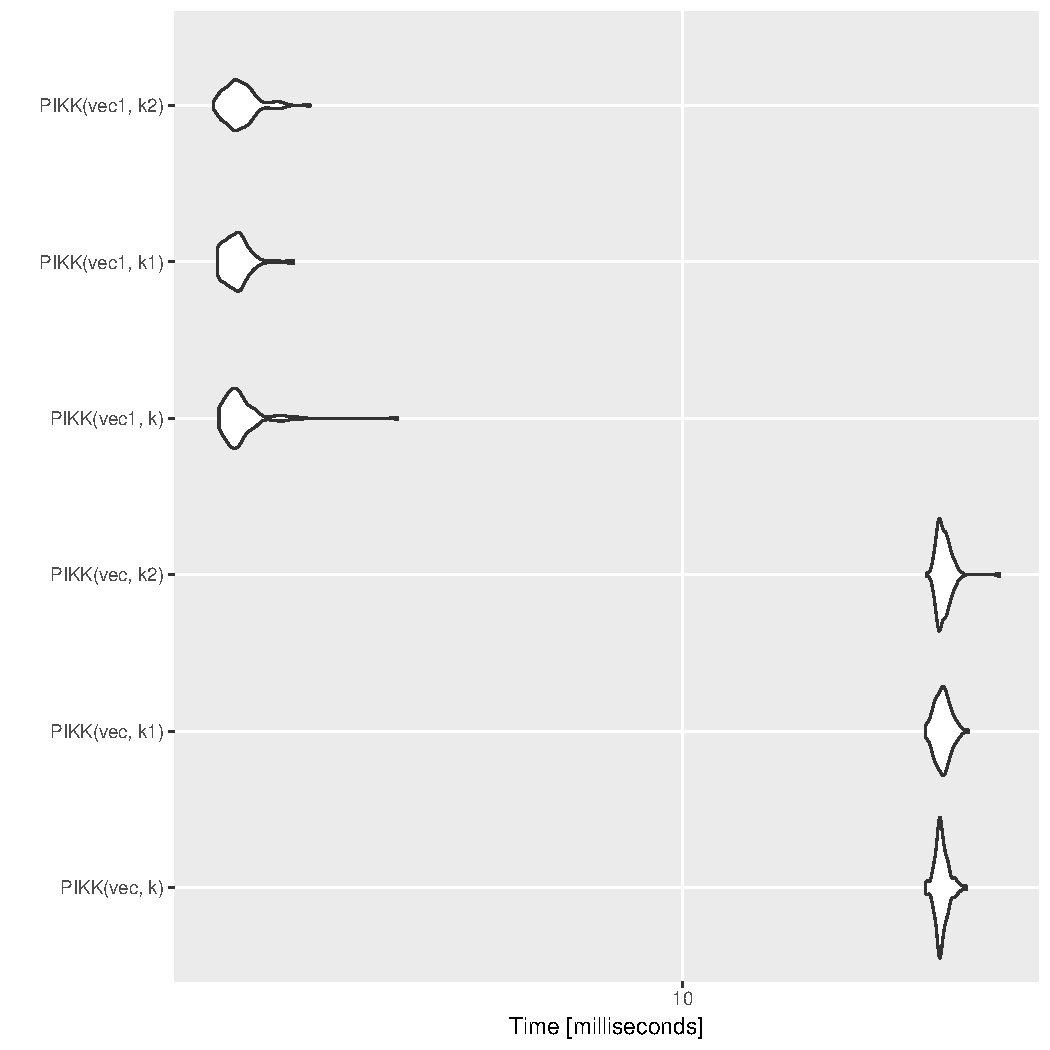
\includegraphics[width=\maxwidth]{figure/unnamed-chunk-12-1} 
\begin{kframe}\begin{alltt}
\hlkwd{autoplot}\hlstd{(new_func)}
\end{alltt}
\end{kframe}
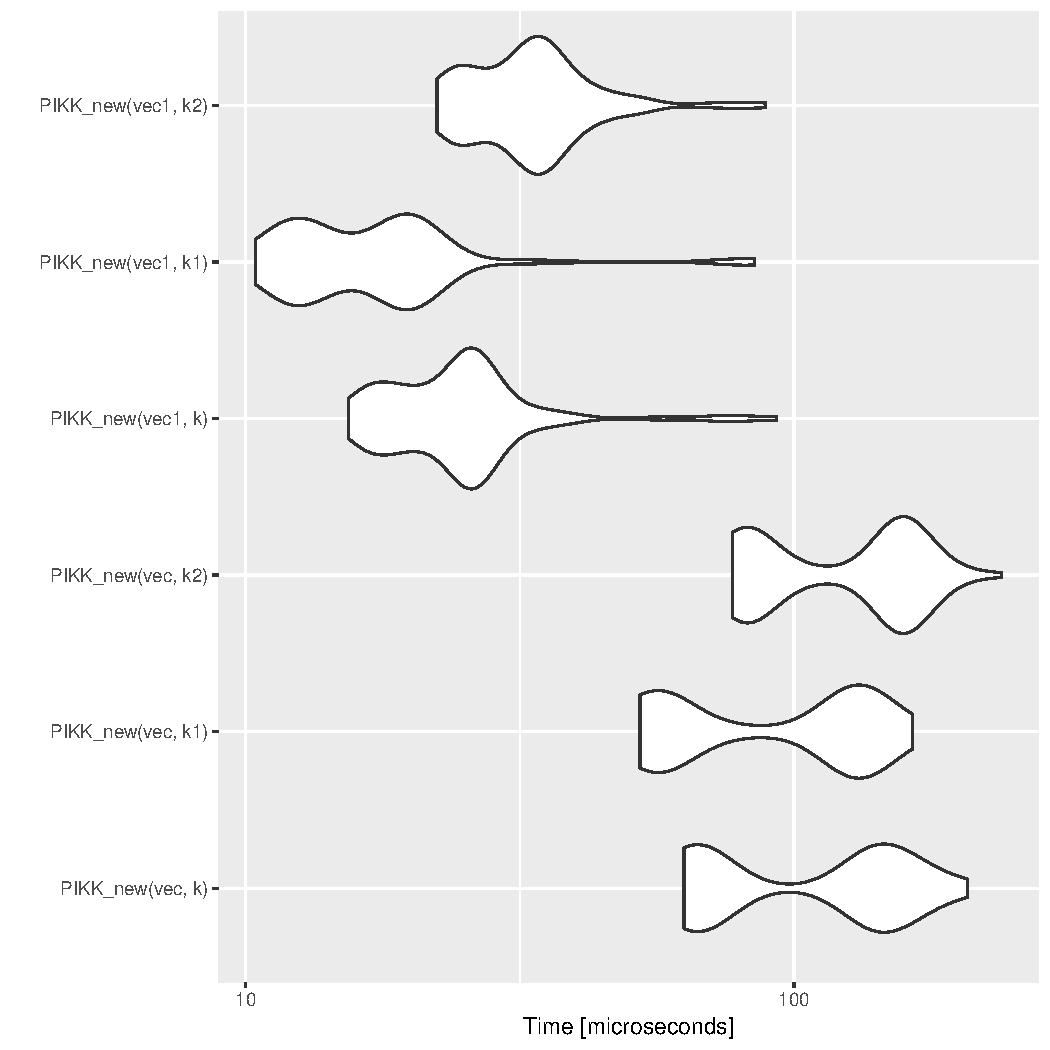
\includegraphics[width=\maxwidth]{figure/unnamed-chunk-12-2} 

\end{knitrout}
From the plots, it is clear that invoking the \emph{sample()} function in the new function drastically increases the speed of completion compared to the original.  The bottleneck of the original \emph{PIKK} function is at the sorting step where the randomly generated distribution is sorted and the indices are taken from the lowest values in that vector.  Removing that increases the efficiency of execution of the code.
\end{document}
